\section{Background}
\label{sec:back}
Content Security Policy (CSP) helps to detect and mitigate attacks
such as Cross-site scripting(XSS) and Clickjacking.
 
\subsection{Cross-site Scripting (XSS)}
Cross-site Scripting (XSS) or script injection is well known
vulnerability in web applications. According to Web Hacking Incident
Database (WHID) 2010 semiannual report, XSS was in the top in the list
of application security risks~\cite{WHID-2010report}.  In XSS attack
malicious script is injected into an otherwise trusted web page
violating integrity of infected web application and causing an
unexpected behavior such as stealing sensitive information or
modifying server side state of a user. When a user visits a web page
of trusted site that contains malicious injected script, the injected
script is executed in user's browser with the principle of trusted
site. Therefore, injected scripts have full control over the session and
thus can send arbitrary requests with valid session and security
tokens.

\begin{figure}[h!]
\begin{center}
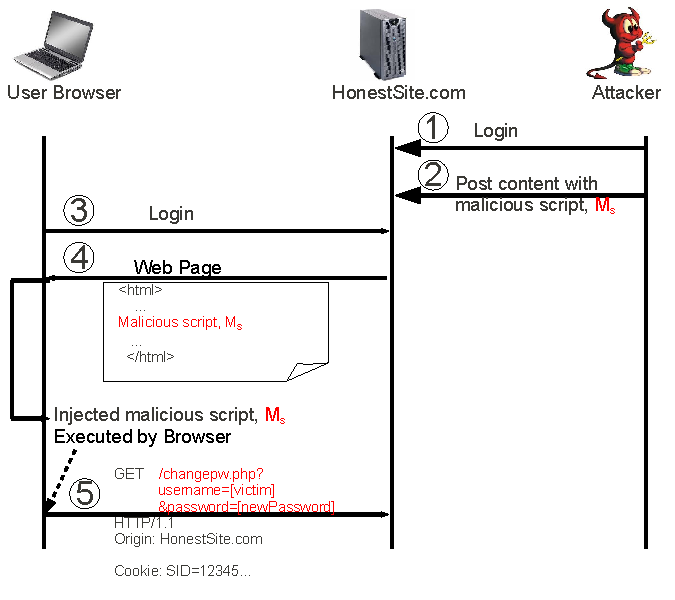
\includegraphics[width=0.5\textwidth]{xss-example}
\end{center}
\caption{Illustration of Cross-Site Scripting}
\label{fig:xssIll}
\end{figure}

\paragraph{\bf An Example of XSS Attack.}
If user visits a web page of vulnerable trusted web site, say {\em
  HonestSite.com} in which attacker has injected inline malicious
script, say $M_{s}$. Malicious script, $M_s$, is executed in the
context of web site and can send state modifying request to {\em
  HonestSite.com}

As shown in Figure~\ref{fig:xssIll}, attacker first login to a web
site, {\em HonestSite.com} (Step 1). On the vulnerable web page of the
web site, attacker submits malicious script, $M_s$ (Step 2). When user
login to the web site (Step 3), and visits the vulnerable web page
(Step 4), injected malicious script, $M_s$ is executed in the context
of web site. When injected script executed in the context of web site
it will compromise the integrity of web site by sending malicious
request to modify user state of the user on the web site (Step
5). Request is generated by injected script running with the principle
of web site and carries valid authentication token, therefore web site
processes the malicious request.

\paragraph{\bf Mitigation of Cross-site Scripting(XSS).}
Content security policy allows website administrators to eliminate
their XSS attack surface. To achieve this goal, CSP allows website
administrators specify which domains the browser should treat as valid
sources of script. Moreover, the web browser will only execute script
in source files from the white-listed domains and will disregard
everything else, including inline scripts.

\subsection{Clickjacking}
In Clickjacking attacks~\cite{nex08,sectheory08}, attackers exploit
the layout feature introduced by iFrames. Specifically, they load a
victim web page into an iFrame on the top and make it
transparent. Then they load a deceptive page in another iFrame at the
bottom layer to attract users to click.

\paragraph{\bf An Example of Clickjacking.}

\begin{figure}[h!]
\begin{center}
\fbox{\parbox{\columnwidth}{
    {\tt
%%\begin{verbatim}
\textless -- Page from www.Websitename.com --\textgreater

<html>

...

<iframe id="victim" src="http://example.com" scrolling="no" 

\hspace*{1.0cm}width="600px" height="600px" style="opacity:0; 

\hspace*{1.0cm}position:absolute; left:10px; top:10px;">

</iframe>

...

<div style = "position:absolute; top:Ypx;left:Xpx;">

\hspace*{1.0cm}<a href= "http://example.com">Click Here</a>

</div>

...

</html>
%%\end{verbatim}
}
}}
\end{center}
  \vspace{-0.3in}
\caption{\small Clickjacking using transparent iFrame and overlay objects.}
\label{fig:clickGuardoverlayobject}
\end{figure}


\begin{figure}[h!]
\begin{center}
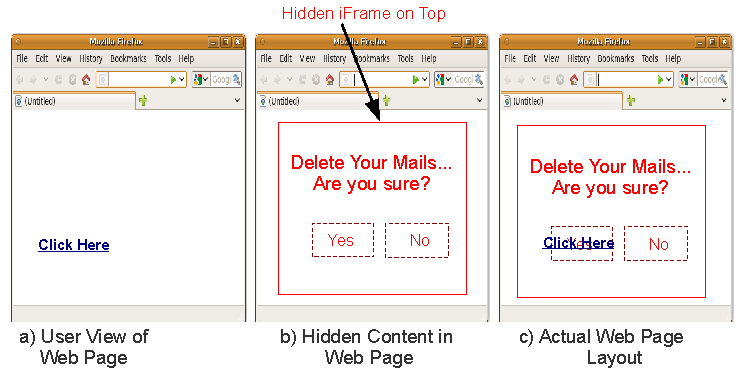
\includegraphics{overlayExa}
\end{center}
  \vspace{-0.3in}
\caption{\small Illustration of Clickjacking using transparent iFrame
  and overlay objects}
\label{fig:clickGuardoverlayobjectIll}
\end{figure}

Figure~\ref{fig:clickGuardoverlayobject} shows an example of a
Clickjacking attack. The front page of {\tt http://example.com} is
loaded inside a transparent iFrame (zero opacity value to make it
transparent). To lure users to click at a particular location of the
page loaded inside the transparent iFrame, the attacker creates a link
in the visible bottom layer, which is located exactly at the same
position where the attacker wants users to click in the top layer. As
shown in Figure~\ref{fig:clickGuardoverlayobject}, the attacker
specifies the location of a link by setting its X and Y
coordinates. When users try to click on the link, they actually click
on the transparent layer of the iFrame loaded with the page from {\tt
  example.com}. An illustration of such a Clickjacking attack is
presented in Figure~\ref{fig:clickGuardoverlayobjectIll}.


\paragraph{\bf Mitigation of Clickjacking.}
Content Security Policy enables a protected website {\tt S} to specify
which websites can embed {\tt S}. That is, a protected website {\tt S}
can decide what other websites it trusts to embed it.
